\documentclass[11pt]{article}
\usepackage[utf8]{inputenc}
\usepackage{minimalist}
\usepackage{graphicx}
\usepackage{multicol}
\usepackage{array}

\title{\textbf{Matrice}\\[4pt]\large Predavanje 10}
\author{iobih škola}
\date{}

\begin{document}
\maketitle
\thispagestyle{fancy}
\markboth{Matrice — Predavanje 10}{}

% ═════════════════════════════════════════════════════════════════════════
\section*{Zagrijavanje: Leksikografski redoslijed}

Možemo li uporediti dvije riječi znakovima $>$ i $<$? Na prvu možda nije
logično, ali odgovor je da! Ako imamo dvije riječi $X$ i $Y$, veća je ona koja
bi došla kasnije u rječniku. To zovemo leksikografskim poređenjem.

Kako bismo utvrdili koja riječ dolazi prije u rječniku vršimo poređenje slovo po slovo, s lijeva na desno:

\begin{enumerate}
    \item Nađi prvu poziciju na kojoj se slova razlikuju.
          Koja god riječ ima \emph{abecedno manje} slovo na toj poziciji — ta dolazi prva.
    \item Ako se jedna riječ završi a razlike još nema — \emph{kraća} dolazi prva.
    \item Ako ne postoji razlika niti među slovima niti u dužini riječi, one su jednake.
\end{enumerate}

\begin{center}
\begin{tabular}{@{} >{\ttfamily}l l l @{}}
    \toprule
    \textbf{Poređenje} & \textbf{Razlika} & \textbf{Rezultat} \\
    \midrule
    "suncokret" vs "zub" & pozicija 0: \texttt{s} < \texttt{z} & "suncokret" $<$ "zub" \\
    "ajvar" vs "avion"  & pozicija 1: \texttt{j} < \texttt{v} & "ajvar" $<$ "avion" \\
    "drvo"  vs "drvored" & "drvo" je prefiks, kraće & "drvo" $<$ "drvored" \\
    \bottomrule
\end{tabular}
\end{center}

\smallskip
U C++-u, stringovi se porede operatorima \texttt{<}, \texttt{>}, \texttt{==}
i automatski koriste leksikografski redoslijed:

\begin{lstlisting}
string a = "ajvar", b = "avion";
if (a < b) cout << a << " dolazi prije " << b;
\end{lstlisting}

\newpage

% ═════════════════════════════════════════════════════════════════════════
\section*{Primjer iz pravog svijeta: Simulacije šumskih požara}

Jedna od čestih upotreba programiranja jeste u svrhu izvršavanja simulacija rijetkih/opasnih događaja 
kako bismo se znali za njih što bolje pripremiti. Jedan od zanimljivih primjera simulacija jesu simulacije
šumskih požara.


\begin{zaradoznale}
    Postoje razni alati za praćenje i simulacije šumskih požara na internetu; evo jedan primjer:
    \href{https://wildfire.concord.org/}.
    Evo i jedan zanimljiv video o matematici iza šumskih požara: 
    \href{https://www.youtube.com/watch?v=HBluLfX2F\_k}
\end{zaradoznale}


Šumu možemo predstaviti kao tabelu u kojoj svako polje prestavlja poziciju na karti. Svako polje
\texttt{karta[r][k]} ima jedno od četiri stanja:

\begin{center}
\begin{tabular}{@{} c l l @{}}
    \toprule
    \textbf{Znak} & \textbf{Stanje} & \textbf{Opis} \\
    \midrule
    \texttt{.} & Prazno     & Golo tlo — vatra se ne može širiti \\
    \texttt{T} & Drvo       & Živo drvo, može se zapaliti \\
    \texttt{*} & Gori       & Drvo gori ovaj vremenski korak \\
    \texttt{x} & Izgorjelo  & Pepeo, vatra je završena \\
    \bottomrule
\end{tabular}
\end{center}


\begin{figure}[h]
    \centering
    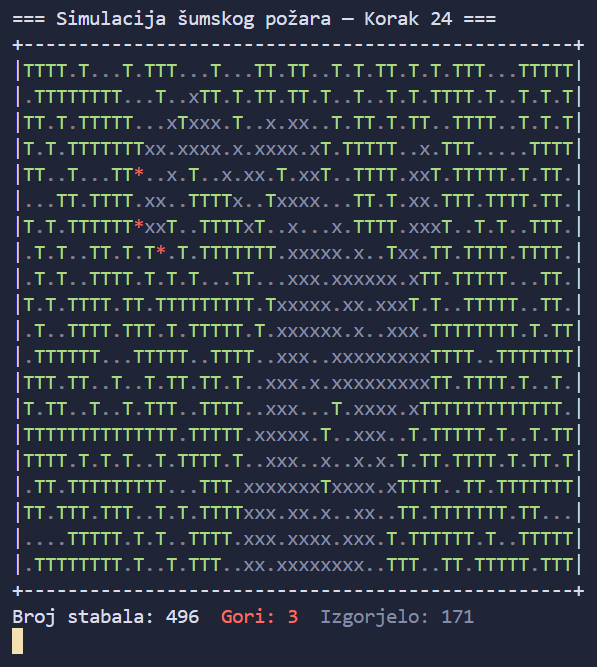
\includegraphics[width=0.5\linewidth]{image.png}
    \caption{C++ program za jednostavnu simulaciju}
    \label{fig:placeholder}
\end{figure}

Na svakom koraku promijenimo kartu prema narednim pravilima: zapaljen element postaje pepeo,
a svaki susjedni element koji sadrži \texttt{DRVO} se pali sa nekom vjerovatnoćom:

\begin{lstlisting}
sljedeca = karta

for (int r = 0; r < REDOVI; r++) {
    for (int k = 0; k < KOLONE; k++) {
        if (karta[r][k] != GORI) continue;

        sljedeca[r][k] = IZGORJELO;

        // Prolazimo kroz sve susjede trenutnog polja
        for (int sr = r-1; sr <= r+1; sr++) {
            for (int sk = k-1; sk <= k+1; sk++) {
                // Preskociti susjeda ako je jednak trenutnom polju
                if (sr == r && sk == k) continue;
                
                // Preskoci polje ako je izvan granica sume
                if (sr < 0 || sr >= REDOVI || sk < 0 || sk >= KOLONE) continue;
                
                // Ako je uslov zadovoljen, susjedno drvo ce se zapaliti
                if (karta[sr][sk] == DRVO && /* dodatni uslov */)
                    sljedeca[sr][sk] = GORI;
            }
        }
    }
}

karta = sljedeca;
\end{lstlisting}



\newpage

% ═════════════════════════════════════════════════════════════════════════
\section*{Matrice (2D nizovi, \textit{engl.} matrix)}

Matricu definišemo kao \textbf{vektor vektora}. Broj redova je \texttt{n},
broj kolona je \texttt{m}:

\begin{lstlisting}
// Matrica od n redova i m kolona, inicijalno popunjena nulama
vector<vector<int>> matrica(n, vector<int>(m, 0));
\end{lstlisting}

\medskip
Čitanje matrice s ulaza radi se sa dvije ugniježdene petlje —
vanjska prolazi kroz \textbf{redove}, unutarnja kroz \textbf{kolone}:

\begin{lstlisting}
int n, m;
cin >> n >> m;

vector<vector<int>> matrica(n, vector<int>(m));

for (int i = 0; i < n; i++) {
    for (int j = 0; j < m; j++) {
        cin >> matrica[i][j];
    }
}
\end{lstlisting}

\begin{napomena}
    Elementi na ulazu ne moraju biti u istom redu — \texttt{cin} automatski
    preskače razmake i nove redove. Dakle, ulaz možeš pisati red po red ili
    sve u jednom redu.
    Npr. u gornjem kodu, naredni ulazi predstavljaju istu matricu: \\
    \texttt{2 3}\\
    \texttt{1 2 3}\\
    \texttt{4 5 6}\\
    i \\
    \texttt{2 3}\\
    \texttt{1 2 3 4 5 6}
\end{napomena}


\newpage

% ═════════════════════════════════════════════════════════════════════════
\section*{Zadaci}


\begin{zadatak}{1 — Razlika dijagonala}
Data je kvadratna matrica dimenzija $n \times n$.
Izračunaj apsolutnu razliku sume \emph{glavne dijagonale}
(elementi $i = j$) i sume \emph{sporedne dijagonale}
(elementi $i + j = n - 1$).

\medskip
\begin{minipage}[t]{0.45\textwidth}
\textbf{Ulaz}\\[2pt]
U prvom redu broj $n$.\\
U narednih $n$ redova, po $n$ cijelih brojeva.

\medskip
\textbf{Izlaz}\\[2pt]
Jedan cijeli broj — apsolutna razlika suma dviju dijagonala.
\end{minipage}
\hfill
\begin{minipage}[t]{0.48\textwidth}
\textbf{Primjer}\\[2pt]
\begin{tabular}{@{}ll@{}}
\textit{Ulaz} & \textit{Izlaz} \\
\begin{minipage}[t]{2.5cm}
\ttfamily\small
3\\
1 2 3\\
4 5 6\\
7 8 9
\end{minipage}
&
\begin{minipage}[t]{2cm}
\ttfamily\small
0
\end{minipage}
\end{tabular}

\medskip
Glavna: $1{+}5{+}9=15$, sporedna: $3{+}5{+}7=15$, razlika: $|15-15|=0$.
\end{minipage}
\end{zadatak}

\begin{zadatak}{2 — Magični kvadrat}
Data je kvadratna matrica dimenzija $n \times n$.
Ispiši sumu svakog reda, sumu svake kolone, te sumu
\emph{glavne dijagonale} (elementi za koje vrijedi $i = j$).

\medskip
\begin{minipage}[t]{0.45\textwidth}
\textbf{Ulaz}\\[2pt]
U prvom redu broj $n$.\\
U narednih $n$ redova, po $n$ cijelih brojeva.

\medskip
\textbf{Izlaz}\\[2pt]
$n$ redova za sume redova,\\
$n$ redova za sume kolona,\\
jedan red za sumu dijagonale.
\end{minipage}
\hfill
\begin{minipage}[t]{0.48\textwidth}
\textbf{Primjer}\\[2pt]
\begin{tabular}{@{}ll@{}}
\textit{Ulaz} & \textit{Izlaz} \\
\begin{minipage}[t]{3cm}
\ttfamily\small
3\\
2 7 6\\
9 5 1\\
4 3 8
\end{minipage}
&
\begin{minipage}[t]{4.5cm}
\ttfamily\small
Suma reda 0 je 15\\
Suma reda 1 je 15\\
Suma reda 2 je 15\\
Suma kolone 0 je 15\\
Suma kolone 1 je 15\\
Suma kolone 2 je 15\\
Suma dijagonale je 15
\end{minipage}
\end{tabular}
\end{minipage}
\end{zadatak}

\begin{zadatak}{3 — Zatočen}
Mačak Cicko se nalazi u tabeli dimenzija $n \times m$.
Ćelije su ili slobodne (\texttt{.}) ili zidovi (\texttt{\#}).
Cicko je na poziciji $(r, k)$ (indeksirano od 0).
Da li je Cicko zatočen, tj.\ da li su sve ćelije oko njega zidovi?

\medskip
\begin{minipage}[t]{0.45\textwidth}
\textbf{Ulaz}\\[2pt]
Red sa $n$ i $m$.
Narednih $n$ redova, svaki sa $m$ karaktera
(\texttt{.} ili \texttt{\#}).
Red sa pozicijom $r$ i $k$.

\medskip
\textbf{Izlaz}\\[2pt]
\texttt{Cicko je zatocen :(}\\
ili\\
\texttt{Cicko nije zatocen :)}
\end{minipage}
\hfill
\begin{minipage}[t]{0.48\textwidth}
\textbf{Primjer}\\[2pt]
\begin{tabular}{@{}ll@{}}
\textit{Ulaz} & \textit{Izlaz} \\
\begin{minipage}[t]{2.5cm}
\ttfamily\small
3 3\\
\#\#\#\\
\#\#\#\\
\#\#\#\\
1 1
\end{minipage}
&
\begin{minipage}[t]{3.5cm}
\ttfamily\small
Cicko je zatocen :(
\end{minipage}
\end{tabular}

\medskip
\begin{tabular}{@{}ll@{}}
\textit{Ulaz} & \textit{Izlaz} \\
\begin{minipage}[t]{2.5cm}
\ttfamily\small
3 3\\
\#\#\#\\
.\#\#\\
\#\#\#\\
1 1
\end{minipage}
&
\begin{minipage}[t]{3.5cm}
\ttfamily\small
Cicko nije zatocen :)
\end{minipage}
\end{tabular}
\end{minipage}
\end{zadatak}

\begin{zadatak}{4 — Ogledalo}
Data je matrica dimenzija $n \times m$.
Napravi \emph{horizontalno zrcaljenje} — svaki red okreni naopako.
Ispiši zrcaljenu matricu, a ispod nju ispiši originalnu i zrcaljenu matricu
jednu pored druge (spojene u isti red).

\medskip
\begin{minipage}[t]{0.45\textwidth}
\textbf{Ulaz}\\[2pt]
Red sa $n$ i $m$.\\
Narednih $n$ redova, po $m$ cijelih brojeva.

\medskip
\textbf{Izlaz}\\[2pt]
Zrcaljena matrica,\\
prazan red,\\
matrica \textquotedblleft spojena\textquotedblright\ (original~|~zrcaljena).
\end{minipage}
\hfill
\begin{minipage}[t]{0.48\textwidth}
\textbf{Primjer}\\[2pt]
\begin{tabular}{@{}ll@{}}
\textit{Ulaz} & \textit{Izlaz} \\
\begin{minipage}[t]{2.5cm}
\ttfamily\small
2 3\\
1 2 3\\
4 5 6
\end{minipage}
&
\begin{minipage}[t]{3.5cm}
\ttfamily\small
3 2 1\\
6 5 4\\
\\
1 2 3 3 2 1\\
4 5 6 6 5 4
\end{minipage}
\end{tabular}
\end{minipage}
\end{zadatak}

% ═════════════════════════════════════════════════════════════════════════
% \section*{Domaća Zadaća}

% \begin{mdframed}[linecolor=accent!40, linewidth=0.8pt, backgroundcolor=accent!3,
%                  innertopmargin=80pt, innerbottommargin=12pt]
%     \color{gray}\small\textit{[Domaća zadaća — dodati naknadno]}
% \end{mdframed}

\end{document}
